Como se comprueba en las pruebas, al emplear \texttt{MPI} sobre este problema no se obtiene ningún beneficio. Por ello, se aplicará \texttt{OpenMP} sobre el algoritmo secuencial en vez de hacerlo sobre el código paralelizado con \texttt{MPI}.

Como se había aclarado en el apartado de \texttt{MPI}, hay partes de nuestro programa que no son paralelizables (o con una complejidad demasiado elevada para el objetivo de este curso). A continuación se muestran partes del código sobre las que sí se puede aplicar \texttt{OpenMP}.

Al inicializar el array, por ejemplo, podemos dividir el trabajo entre varios threads.
\lstinputlisting[language=C]{./src/inicializacion_openmp.c}

Al hallar el máximo elemento del array también se nota mejoría al utilizar varios hilos.
\lstinputlisting[language=C]{./src/maximo_openmp.c}

Por último, al copiar los datos del array auxiliar \emph{b} en el array principal \emph{a} podemos usar varios hilos, ya que los datos no se pisan.
\lstinputlisting[language=C]{./src/copia_datos.c}


Aplicando estas pequeñas modificaciones se aprecia una gran mejora en el tiempo de ejecución con respecto al original (Figura \ref{Comparacion_tiempos} y Figura \ref{Comparacion_speedups}), y eso que la parte principal no se puede paralelizar (la que hace uso del bucket).

\begin{figure}[h!]
	\centering
	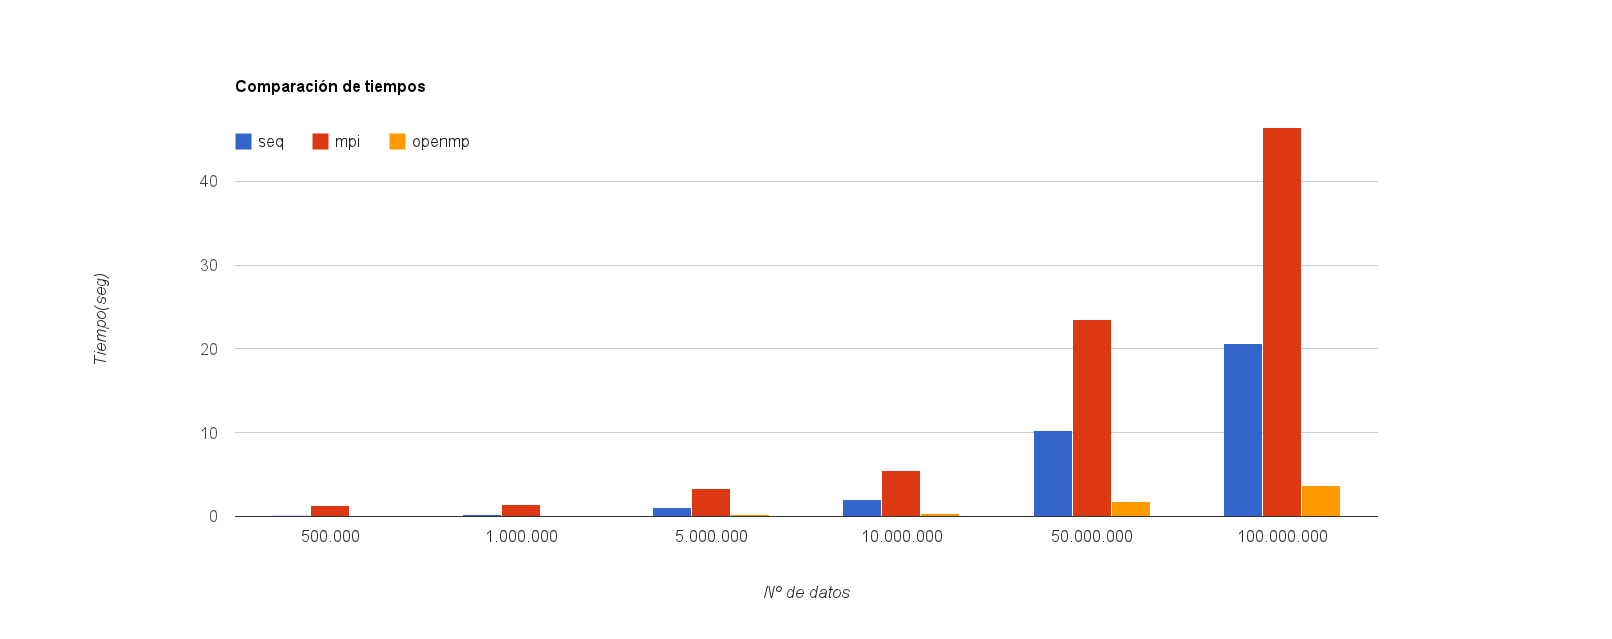
\includegraphics[width=1.3\textwidth]{./res/Comparacion_tiempos}
	\caption{Comparación tiempos}
	\label{Comparacion_tiempos}
\end{figure}

\begin{figure}[h!]
	\centering
	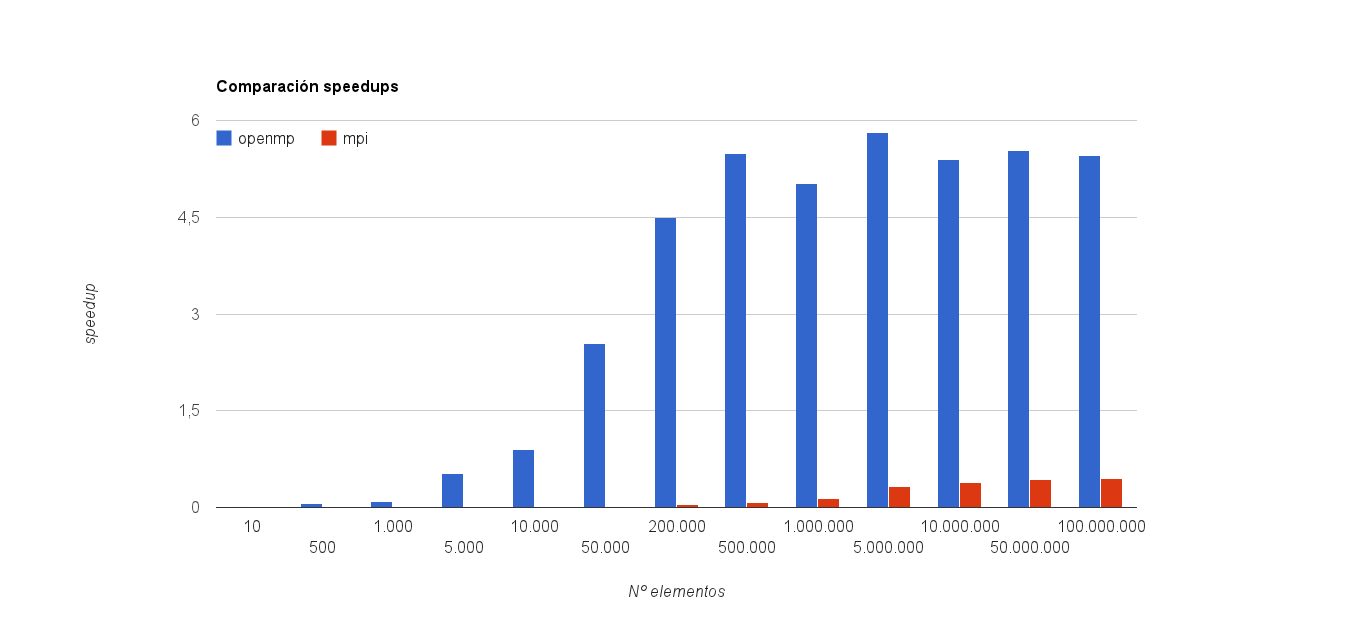
\includegraphics[width=1.3\textwidth]{./res/Comparacion_speedups}
	\caption{Comparación speedups}
	\label{Comparacion_speedups}
\end{figure}